

\tikzset{every picture/.style={line width=0.75pt}} %set default line width to 0.75pt        

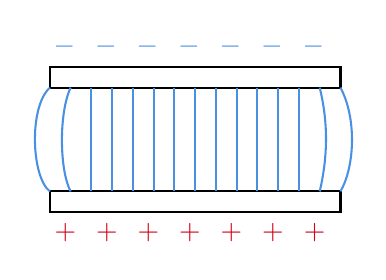
\begin{tikzpicture}[x=0.75pt,y=0.75pt,yscale=-1,xscale=1]
%uncomment if require: \path (0,300); %set diagram left start at 0, and has height of 300

%Shape: Rectangle [id:dp8330327862399476] 
\draw   (100,110) -- (240,110) -- (240,120) -- (100,120) -- cycle ;
%Shape: Rectangle [id:dp5040846084428225] 
\draw   (100,170) -- (240,170) -- (240,180) -- (100,180) -- cycle ;
%Straight Lines [id:da26732252708911663] 
\draw [color={rgb, 255:red, 74; green, 144; blue, 226 }  ,draw opacity=1 ]   (120,120) -- (120,170) ;


%Straight Lines [id:da0361535767352088] 
\draw [color={rgb, 255:red, 74; green, 144; blue, 226 }  ,draw opacity=1 ]   (130,120) -- (130,170) ;


%Straight Lines [id:da8817020598123642] 
\draw [color={rgb, 255:red, 74; green, 144; blue, 226 }  ,draw opacity=1 ]   (180,120) -- (180,170) ;


%Straight Lines [id:da5520456301460932] 
\draw [color={rgb, 255:red, 74; green, 144; blue, 226 }  ,draw opacity=1 ]   (170,120) -- (170,170) ;


%Straight Lines [id:da21245697348265646] 
\draw [color={rgb, 255:red, 74; green, 144; blue, 226 }  ,draw opacity=1 ]   (160,120) -- (160,170) ;


%Straight Lines [id:da5753095290308645] 
\draw [color={rgb, 255:red, 74; green, 144; blue, 226 }  ,draw opacity=1 ]   (150,120) -- (150,170) ;


%Straight Lines [id:da10306217312363986] 
\draw [color={rgb, 255:red, 74; green, 144; blue, 226 }  ,draw opacity=1 ]   (140,120) -- (140,170) ;


%Straight Lines [id:da803418354374354] 
\draw [color={rgb, 255:red, 74; green, 144; blue, 226 }  ,draw opacity=1 ]   (190,120) -- (190,170) ;


%Straight Lines [id:da3863169852881563] 
\draw [color={rgb, 255:red, 74; green, 144; blue, 226 }  ,draw opacity=1 ]   (200,120) -- (200,170) ;


%Straight Lines [id:da21928876530419328] 
\draw [color={rgb, 255:red, 74; green, 144; blue, 226 }  ,draw opacity=1 ]   (210,120) -- (210,170) ;


%Straight Lines [id:da6200684445599047] 
\draw [color={rgb, 255:red, 74; green, 144; blue, 226 }  ,draw opacity=1 ]   (220,120) -- (220,170) ;


%Curve Lines [id:da07526910679469512] 
\draw [color={rgb, 255:red, 74; green, 144; blue, 226 }  ,draw opacity=1 ]   (100,120) .. controls (89.8,129.1) and (91,163.1) .. (100,170) ;


%Curve Lines [id:da7986744788671094] 
\draw [color={rgb, 255:red, 74; green, 144; blue, 226 }  ,draw opacity=1 ]   (240,120) .. controls (247.8,134.5) and (247,157.83) .. (240,170) ;


%Curve Lines [id:da12996916070079956] 
\draw [color={rgb, 255:red, 74; green, 144; blue, 226 }  ,draw opacity=1 ]   (110,120) .. controls (104.2,132.3) and (104.6,159.9) .. (110,170) ;


%Curve Lines [id:da5647857103005902] 
\draw [color={rgb, 255:red, 74; green, 144; blue, 226 }  ,draw opacity=1 ]   (230,120) .. controls (234.21,137.22) and (233.87,153.33) .. (230,170) ;



% Text Node
\draw (107,100) node [color={rgb, 255:red, 74; green, 144; blue, 226 }  ,opacity=1 ]  {$\bm{-}$};
% Text Node
\draw (127,100) node [color={rgb, 255:red, 74; green, 144; blue, 226 }  ,opacity=1 ]  {$\bm{-}$};
% Text Node
\draw (147,100) node [color={rgb, 255:red, 74; green, 144; blue, 226 }  ,opacity=1 ]  {$\bm{-}$};
% Text Node
\draw (167,100) node [color={rgb, 255:red, 74; green, 144; blue, 226 }  ,opacity=1 ]  {$\bm{-}$};
% Text Node
\draw (187,100) node [color={rgb, 255:red, 74; green, 144; blue, 226 }  ,opacity=1 ]  {$\bm{-}$};
% Text Node
\draw (207,100) node [color={rgb, 255:red, 74; green, 144; blue, 226 }  ,opacity=1 ]  {$\bm{-}$};
% Text Node
\draw (227,100) node [color={rgb, 255:red, 74; green, 144; blue, 226 }  ,opacity=1 ]  {$\bm{-}$};
% Text Node
\draw (107.5,190) node [color={rgb, 255:red, 208; green, 2; blue, 27 }  ,opacity=1 ]  {$\bm{+}$};
% Text Node
\draw (127.5,190) node [color={rgb, 255:red, 208; green, 2; blue, 27 }  ,opacity=1 ]  {$\bm{+}$};
% Text Node
\draw (147.5,190) node [color={rgb, 255:red, 208; green, 2; blue, 27 }  ,opacity=1 ]  {$\bm{+}$};
% Text Node
\draw (167.5,190) node [color={rgb, 255:red, 208; green, 2; blue, 27 }  ,opacity=1 ]  {$\bm{+}$};
% Text Node
\draw (187.5,190) node [color={rgb, 255:red, 208; green, 2; blue, 27 }  ,opacity=1 ]  {$\bm{+}$};
% Text Node
\draw (207.5,190) node [color={rgb, 255:red, 208; green, 2; blue, 27 }  ,opacity=1 ]  {$\bm{+}$};
% Text Node
\draw (227.5,190) node [color={rgb, 255:red, 208; green, 2; blue, 27 }  ,opacity=1 ]  {$\bm{+}$};


\end{tikzpicture}
